%A LaTeX model for SYSU General Phys. Lab. by Probfia Gao.
%用XeLaTeX编译
\documentclass[11pt,a4paper]{ctexart}

%在下面补全实验名，例如 实验BB3 光电效应实验。
\newcommand{\ExpeName}{实验D4-1 电子顺磁共振实验}

\usepackage{fancyhdr}
\usepackage{amsmath}
\usepackage{graphicx}
\usepackage[hmargin=1.25in,vmargin=1in]{geometry}
\usepackage{pdfpages}
\usepackage[colorlinks,
            linkcolor=red,
		 urlcolor=black]{hyperref}
\usepackage{cleveref}
\usepackage{float}


\crefname{equation}{}{}
\crefname{figure}{图}{图}
\crefname{footnote}{注释}{注释}
\crefname{table}{表}{表}

%\cpic{<尺寸>}{<文件名>}}用于生成居中的图片。
\newcommand{\cpic}[2]{
\begin{center}
\includegraphics[scale=#1]{#2}
\end{center}
}

%\cpicn{<尺寸>}{<文件名>}{<注释>}用于生成居中且带有注释的图片，其label为图片名。
\newcommand{\cpicn}[3]
{
\begin{figure}[H]
\cpic{#1}{#2}
\caption{#3\label{#2}}
\end{figure}
}

\newcommand{\beq}{\begin{equation}}
\newcommand{\eeq}{\end{equation}}
\newcommand{\bea}{\begin{equation}\begin{aligned}}
\newcommand{\eea}{\end{aligned}\end{equation}}

%输入单位和数学常数
%下面所有命令需在公式环境下使用
\newcommand{\e}{\mathrm{e}}   %自然常数e = \e
\newcommand{\im}{\mathrm{i}}   %虚数单位i = \im
\newcommand{\meter}{\mathrm{m}}      %单位/前缀 = \单位/前缀英文名
\newcommand{\newton}{\mathrm{N}}  
\newcommand{\joule}{\mathrm{J}}
\newcommand{\second}{\mathrm{s}}
\newcommand{\gram}{\mathrm{g}}
\newcommand{\ampere}{\mathrm{A}}
\newcommand{\kilo}{\mathrm{k}}
\newcommand{\milli}{\mathrm{m}}
\newcommand{\kelvin}{\mathrm{K}}
\newcommand{\mole}{\mathrm{mol}}
\newcommand{\volt}{\mathrm{V}}
\newcommand{\nano}{\mathrm{n}}
\newcommand{\degreeC}{^\circ \mathrm{C}}  %摄氏度符号 = \degreeC

\newcommand{\unit}[1]{\rm \ #1}
\newcommand{\emptyline}{\par \ \\ }

\pagestyle{fancy}

\fancyhead[L]{\footnotesize{中山大学物理与天文学院近代物理实验}}
\fancyhead[R]{\footnotesize{\ExpeName}}
\fancyfoot[C]{\thepage}

\begin{document}
%第一页
\cpic{0.255}{e1}%学生信息和计分表格
\begin{table}[H]
\centering
\begin{tabular}{|p{32mm}|p{32mm}|p{32mm}|p{32mm}|}
\hline
年级、专业： & 17级 物理学 & 组号： & 实验班6 \\ \hline
姓名： & 高寒 & 学号： & 17353019 \\ \hline
日期： & \today & 教师签名： &  \\ \hline
\end{tabular}
\end{table}
\begin{center}
\LARGE\textbf{{\ExpeName}}
\end{center}
\large{【实验报告注意事项】}
\begin{enumerate}
 \item 实验报告由三部分组成：
 \begin{enumerate}
  \item[1)]预习报告：（提前一周）认真研读\textbf{\uline{实验讲义}}，弄清实验原理；实验所需的仪器设备、用具及其使用（强烈建议到实验室预习），完成讲义中的预习思考题；了解实验需要测量的物理量，并根据要求提前准备实验记录表格（由学生自己在实验前设计好，可以打印）。预习成绩低于50\%者不能做实验{\color{red} (实验D2和D3需要提前一周的周四完成预习报告交任课老师批改，批改通过后，才允许做实验)}。

  \item[2)]实验记录：认真、客观记录实验条件、实验过程中的现象以及数据。实验记录请用珠笔或者钢笔书写并签名（{\color{red}用铅笔记录的被认为无效}）。{\color{red}保持原始记录，包括写错删除部分，如因误记需要修改记录，必须按规范修改。}（不得输入电脑打印，但可扫描手记后打印扫描件）；离开前请实验教师检查记录并签名。
  \item[3)]分析讨论：处理实验原始数据（学习仪器使用类型的实验除外），对数据的可靠性和合理性进行分析；按规范呈现数据和结果（图、表），包括数据、图表按顺序编号及其引用；分析物理现象（含回答实验思考题，写出问题思考过程，必要时按规范引用数据）；最后得出结论。
 \end{enumerate}
 \textbf{实验报告}就是预习报告、实验记录、和数据处理与分析合起来，加上本页封面。
 \item 每次完成实验后的一周内交\textbf{实验报告}。
 \item 除实验记录外，实验报告其他部分建议双面打印。
\end{enumerate}
\ 
\\
\ 


\begin{flushright}                                                           %模板作者
\tiny{
A \LaTeX \ model for Modern Phys. Lab., SPA, SYSU by \em{\href{https://www.weibo.com/3532532974/profile?rightmod=1&wvr=6&mod=personinfo&is_all=1}{Probfia} Gao.}
}
\end{flushright}

\includepdf[pages=2-14]{preview.pdf}
\iffalse
\newpage%预习报告
\begin{center}
\LARGE{\textbf{\ExpeName}}
\end{center}
\textbf{【实验目的】}
\begin{enumerate}
 \item[1.] (目的1)
 \item[2.] (目的2)
\end{enumerate}
\textbf{【仪器用具】}
%将讲义中的表格截图保存为t1在该文件夹下后删去下一行之前的%符号，合理调整scale参数。
%cpic{0.3}{t1}
%或者自己去 https://www.tablesgenerator.com/ 做一个表。
\textbf{【原理概述】}\par
该实验\\
\textbf{【实验前思考题】}
\begin{enumerate}
 \item[1.] (问题1)
 \item[2.] (问题2)
\end{enumerate}

\newpage%实验记录
%\cpic{0.255}{e2}%学生信息表格
\begin{table}[H]
\centering
\begin{tabular}{|p{32mm}|p{32mm}|p{32mm}|p{32mm}|}
\hline
年级、专业： & 17级 物理学 & 组号： & 实验班6 \\ \hline
姓名： & 高寒 & 学号： & 17353019 \\ \hline
日期： &  & 实验地点： & 珠海教学楼 A102 \\ \hline
学生签名： &  
\includegraphics[scale=0.09]{sign}& 评分： &  \\ \hline
日期： &  & 教师签名： &  \\ \hline
\end{tabular}
\end{table}

\begin{center}
\LARGE{\textbf{\ExpeName}}
\end{center}
\textbf{【实验内容、步骤、结果】}
\par
(表格)
\newline
\textbf{【实验过程中遇到问题记录】}\par
\cpic{0.81}{none}
\fi
%生成最终报告时将上面内容全部删除或注释（用\iffalse \fi），将扫描得到的实验报告保存为Record.pdf在LaTeX model for GPL下，将下行命令的注释号删去。注意根据实际页数调整pages参数。

\includepdf[pages=1-3]{Record}


\newpage%分析与讨论
%\cpic{0.255}{e3}%学生信息表格
\begin{table}[H]
\centering
\begin{tabular}{|p{32mm}|p{32mm}|p{32mm}|p{32mm}|}
\hline
年级、专业： & 17级 物理学 & 组号： & 实验班6 \\ \hline
姓名： & 高寒 & 学号： & 17353019 \\ \hline
日期： & \today &  &  \\ \hline
评分： &  & 教师签名： &  \\ \hline
\end{tabular}
\end{table}
\begin{center}
\LARGE\textbf{{\ExpeName}}
\end{center}
\textbf{【分析与讨论】}\\
1.\textbf{励磁线圈电压-磁场强度标定}
\par
将得到的电压-磁场强度数据绘制成散点图，绘出回归直线如\cref{fit_lin}。
\cpicn{0.6}{fit_lin}{标定数据回归直线}
将数据代入回归直线的斜率、截距公式，得到电压-磁场关系为
\beq \label{rel}
B = 3224.44 + 24.03V \unit{Gs}
\eeq
截距和斜率的标准差为\cite{error}
\bea
\sigma_b &= 0.59\unit{Gs} \\
\sigma_k &= 0.41\unit{Gs/V}
\eea
当励磁线圈上的电压为$V$时，$B$的标准偏差由误差传递公式给出
\beq
\sigma_B = \sqrt{(0.41V)^2 + 0.59^2} = \sqrt{0.1681 V^2+0.3481}\unit{(Gs})
\eeq
此后的实验中可以直接由励磁线圈上加的电压得到线圈中心附近的磁场。
\emptyline
2.\textbf{电子自旋共振信号}
\par
调节短路活塞，使得直流电压最小后，将示波器调到交流档位，观察到此时的波形如\cref{os1}。
\cpicn{0.09}{os1}{最初的波形}
其中黄线为测得的信号，蓝线为扫描电源的信号，可以看到，两者是同频率的。
\par
进一步增大磁场，得到的波形如\cref{os2}、\cref{os3}、\cref{os4}、\cref{os5}、\cref{os6}。
\cpicn{0.09}{os2}{逐渐增大励磁线圈电压得到的波形}
\cpicn{0.09}{os3}{逐渐增大励磁线圈电压得到的波形}
\cpicn{0.09}{os4}{逐渐增大励磁线圈电压得到的波形}
\cpicn{0.09}{os6}{逐渐增大励磁线圈电压得到的波形}
\cpicn{0.09}{os5}{逐渐增大励磁线圈电压得到的波形}
可以看到，在\cref{os5}中，已经出现了共振信号的踪迹，即吸收信号与扫描信号频率比为$2:1$的趋势\cite{lec}。
\par
此时条件扫描信号，使得共振信号在扫描信号一个周期内的两个峰等间距，如\cref{os7}，
\cpicn{0.09}{os7}{电子自旋共振信号}
此时的李萨如图如\cref{ls1}、\cref{ls2}。
\cpicn{0.09}{ls1}{电子自旋共振信号出现时的李萨如图}
\cpicn{0.09}{ls2}{电子自旋共振信号出现时的李萨如图}
此时励磁线圈电压为$5.01\unit{V}$。
\par
利用导出数据做得的共振信号曲线和李萨如图如\cref{ren_cur}，\cref{rough_ls}。
\cpicn{0.6}{ren_cur}{导出数据作得的共振信号曲线}
\cpicn{0.6}{rough_ls}{共振时的李萨如图}
可以看到，由于测量信号十分微弱，噪声非常明显。为了平滑噪声的影响，取相邻10个数据点重新作出李萨如图如\cref{smooth_ls}。
\cpicn{0.6}{smooth_ls}{平滑处理后的李萨如图}
可以看到，其纵向最大交点为4，横向为2，体现了共振信号频率与扫描信号频率比为$2:1$的事实。
\emptyline
3.\textbf{DPPH样品的g因子计算}
\par
在如\cref{os7}的电子自旋共振信号出现时，利用\cref{rel}得到此时的磁感应强度为
\beq
B_0 = 3224.44 + 24.03\times 5.01  = 3344.85\unit{(Gs)}
\eeq
不确定度
\beq
\sigma_{B_0} = \sqrt{0.1681 5.01^2+0.3481}= 2.2\unit{(Gs}) 
\eeq
此时旋转频率计，观测到信号出现明显跳动时，频率为
\beq
f = 9.390 \times 10^{9} \unit{Hz}
\eeq
由公式
\beq
f = g \frac{\mu_B}{h} B_0
\eeq
代入$\mu_B = 5.7884 \times 10^{-11} \unit{MeV/Gs}$，$h = 4.1357\times 10^{-21} \unit{MeV\cdot s}$，得到
\beq
g_{\rm DPPH} = \frac{fh}{\mu_B B_0} = \frac{9.390 \times 10^{9} \unit{Hz} \times 4.1357\times 10^{-21} \unit{MeV\cdot s}}{5.7884 \times 10^{-11} \unit{MeV/T} \times 3344.85\unit{Gs} }= 2.0058
\eeq
由误差传递公式
\beq
\sigma_{g_{\rm DPPH}} = g_{\rm DPPH} \frac{\sigma_{B_0}}{B_0} = 0.0012
\eeq
故结果表示为
\beq
g_{\rm DPPH} = 2.0058(12)
\eeq
参考值为$g = 2.0036$，相对误差$\delta = \frac{2.0058-2.0036}{2.0036}=0.11\%$，测量比较准确，且在误差极限范围内。
\emptyline
\\
4.\textbf{横向弛豫时间$T_2$的计算}
\par
实验中测得
\beq
B' = 8.4\unit{Gs}
\eeq
通过导出的数据做吸收曲线如\cref{ren_cur}，随机选取5个峰，得到半高宽
\beq
\Delta t \approx 0.001 \unit{s}
\eeq
磁场差
\bea
\Delta B &= B'( \sin \omega t_2 - \sin \omega t_2)\\
&= 2B' \cos \omega \frac{t_1 + t_2}{2} \sin \omega \frac{t_2 - t_1}{2} \\
&= 2B'\sin \omega \frac{\Delta t}{2}
\eea
其中因为$\frac{t_1 + t_2}{2} = t_0$对应调制信号，$\sin \omega t_0 = 0$，$\cos \omega t_0 = 1$。代入数据得到
\beq
\Delta B \approx 2.628 \unit{Gs}
\eeq
于是，横向弛豫时间估计为
\beq
T_2 = \frac{2}{\gamma \Delta B} \sim 4 \times 10^{-8} \unit{s} \sim 40 \unit{ns}
\eeq

\emptyline
\\
5.\textbf{波导波长和微波波长的计算}
\par
调节远端短路活塞，找到两个相邻的谐振点
\bea
L_1 &= 4.916\unit{mm}\\
L_2 &= 27.308\unit{mm}
\eea
波导波长为
\beq
\lambda_g = 2(L_2-L_1) = 22.392\unit{mm}
\eeq
又临界波长$\lambda_c = 2a = 45.72\unit{mm}$，由
\beq
\lambda_g = \frac{\lambda}{\sqrt{1 - \left( \frac{\lambda}{\lambda_c}\right)^2}}
\eeq
解得微波波长
\beq
\lambda = 18.662\unit{mm}
\eeq
经查电磁波谱\cite{dtem,ced}，这个波长确实在微波对应的波长范围内。
\emptyline
\\
6.\textbf{直接法测量共振吸收信号}\par
以磁场强度为横坐标，信号幅度为纵坐标绘图如\cref{abs_cur}。
\cpicn{0.6}{abs_cur}{直接法测量吸收信号}
可以看到明显的共振吸收现象，第一个较小的峰出现在
\beq
B_1 = 3341.7\unit{Gs}
\eeq
第二个更加显著的峰出现在
\beq
B_2 = 3353.0\unit{Gs}
\eeq
第一个峰与实验主要内容中测得的峰更加接近，第二个峰的出现原因待进一步研究。
\emptyline
\emptyline
\\
\textbf{【实验后思考题】}
\begin{enumerate}
\item {\bf 观察电子自旋共振需要提供哪些磁场？它们各起什么作用？}\par
需要提供一个由励磁线圈提供的恒定匀强磁场$B_0$，它与自旋磁矩相互作用，发生塞曼效应使得原简并的能级分裂\cite{atom,dtaqm}；另由微波提供一个交变磁场，当它的频率由短路活塞调节到与能级差对应的频率$\nu = \frac{\Delta E}{h}$相同时，分裂的能级间发生共振吸收。
\item {\bf 微波谐振腔的作用是什么?腔长和微波频率的关系是什么?调节短路活塞的作用
是什么?实验样品应位于什么位置?为什么?}
\par
微波谐振腔使得交变电磁场在此形成驻波，此时腔长与波导波长满足直线驻波条件\cite{dtem}
\beq
L = \frac{n}{2} \lambda_g
\eeq
微波波长$\lambda$由下式解出
\beq
\lambda_g = \frac{\lambda}{\sqrt{1 - \left(\frac{\lambda}{\lambda_c}\right)^2}}
\eeq
波长与频率的关系
\beq
f = \frac{c}{\lambda}
\eeq
调节短路活塞可以调节腔长从而使驻波条件满足，样品应放在交变电磁场幅值尽可能大的地方检验，此时的实验现象更加明显，易于观察。
\end{enumerate}















\bibliographystyle{IEEEtran}
\bibliography{model.bib}

\end{document}